\section{Analysis}\label{sec:analysis}

Building up on our initial idea and problem formulation, we determine two major functional areas that must be supported by our proposed system:

\begin{itemize}[noitemsep]
    \item \textit{\acrfull{pacs}} (access to restricted premises in a company or institution, building access control etc.)
    \item \textit{Online Access Control} (access to computer systems, applications, online sign-in etc.)
\end{itemize}

While the  typical question in a \acrshort{pacs} would be ``\textit{Is the person allowed to enter beyond this point}?'', and can be controlled by a variety of physical barriers, doors, turn-sites and the like, the online access control is more complex. Enterprises nowadays operate a wide spectrum of software solutions including on-premise applications, legacy systems, cloud-based and \acrshort{saas} applications, internally or externally oriented \acrshort{api}s and databases. All of these require some level of access control. To break down this structure, we first begin by identifying two service classes:
\begin{enumerate*}[label=(\roman*)]
    \item \textit{internal applications}, that sit within the enterprise security realm; and 
    \item \textit{external applications}, that include cloud based software, \acrshort{saas} solutions and partner/vendor applications, and which reside outside the given security realm.
\end{enumerate*}

The external applications can be further divided based on their interactions with the internal systems. Applications that are not business critical and/or are not integrated with the business processes may not require access to protected resources at all. Examples of such applications would be a lunch booking system or a company social network. These would be primarily used by the employees, but would not require connectors to business-critical systems and could therefore reside outside the security realm.

Other external applications, however, may require access to business-critical resources for their functions. \acrlong{crm} or payroll system may both be purchased as a \acrshort{saas}, but both require connectors to the protected resources to properly fulfil their functions. We can therefore extend our classification of the external applications accordingly -- applications that
\begin{enumerate*}[label=(\roman*)]
    \item \textit{require access to protected resources} and
    \item \textit{do not require access to protected resources}.
\end{enumerate*}

The access control of \textit{internal applications} will likely differ from access control of \textit{external applications} and similarly, the access control for applications that require access to protected reources will differ from those that do not. We can therefore devise an access control breakdown chart, as shown in Figure~\ref{fig:acs-classification}. 

Multiple sources list Identification, Authentication and Authorisation as the three basic steps in access control~\cite{Harris2008CISSPGuide, 2018AccessSystems, 2003IdentificationAuthorization}. We focus on strong authentication and authorisation in the system design and describe these further in the following sections.

\begin{figure}[ht]
    \centering
    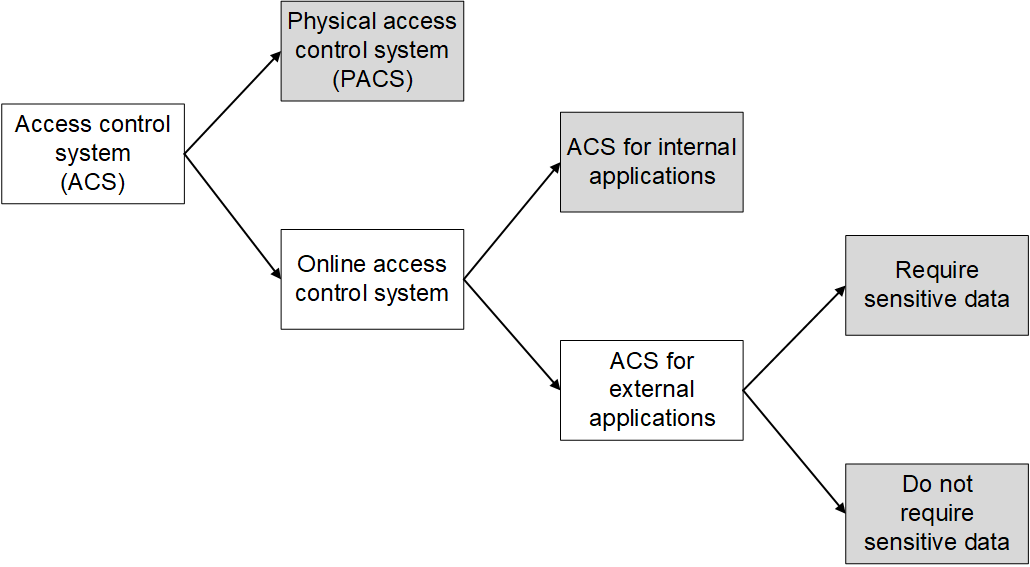
\includegraphics[width=.95\textwidth]{acs-classification}
    \caption{Access control system breakdown chart. \acrshort{acs} for external applications is different for applications work with sensitive data from \acrshort{acs} for external applications that do not work with sensitive data.}
    \label{fig:acs-classification}
\end{figure}

\subsection{Authentication}
In \acrshort{pacs}, physical tokens, such as ID cards, are the common practice nowadays. A survey carried out in 2016 indicated that above 40\% of the companies use low frequency proximity cards as their main method for personal authentication. These cards, operating between 125-134kHz proximity cards are considered an obsolete technology and are not secure~\cite{Hakamaki2015SecurityTechnology}. On the other end of the spectrum, around 20\% of the companies indicated use of mobile devices as a part of their \acrshort{pacs} solution~\cite{HIDGlobal2017TheEnterprise}. 

The main benefit of using a mobile device for this purpose is, that most people already own a smartphone and usually carry it with them at all times. Other technologies represented in the survey that are considered secure today, include iCLASS (contact-less card) and MIFARE DesFire (contact-less card). FIDO, nor FIDO2 keys (NFC, Bluetooth, or other) are not mentioned in the survey, although compatible \acrshort{pacs} systems exist on the market today\footnotemark. 

FIDO and FIDO2 enjoy support of big companies like Google, Facebook and Microsoft, but consumer-oriented application permit the use only as the second authentication factor. Google uses FIDO U2F keys for their employees, but only as a password replacement in the online login scenario~\cite{Krebs2018Google:Phishing} and Microsoft only supports FIDO2 keys with personal Microsoft accounts. As shown in Section~\ref{sec:online-access-control}, even Azure AD does not support this technology. To explore how FIDO2 can be used for hybrid access control on an enterprise scale, we introduce a mandatory support of FIDO2 as a requirement for our system.
% 
\footnotetext{\url{https://web.archive.org/web/20190319221618/https://www.yubico.com/works-with-yubikey/catalog/modis/}, accessed 19 March 2019}

There is already a variate of devices that have been FIDO2 certified, with the Android system being the latest addition to the list~\cite{FIDOAlliance2019AndroidPasswords}. Consideration needs to be put into how the FIDO2 flow will be incorporated in the system and which of the FIDO2-certified devices should be used in the flow. In the \acrshort{pacs}, usability and namely the speed is an important criteria, since existing systems already offer very low- to no-latency during a typical door opening use case. Beyond \acrshort{pacs}, the current access control solutions are above all used for employee identification (as an ID badge)~\cite{HIDGlobal2017TheEnterprise} and the employee is only issued a single badge. The recommended approach in case the employee forgets the badge is to assign a temporary one that can be used during a limited time period and must be returned afterwards~\cite{Ryan2018HowBadges}.

In the online authentication, we can see that the systems support a wider range of authentication (and account recovery) methods, and the user is left to decide, which is authentication method do they prefer. Offering multiple methods simultaneously makes sense for the online access control scenario, because unlike in \acrshort{pacs}, were the on-site reception/security personnel can verify employees identity and issue a temporary badge, in the online access control this is not always possible. In case of forgotten credentials, the identity would therefore needed to be verified remotely (typically over phone), which is not always feasible.

In the proposed hybrid access control system, we must therefore provide an authenticator, that is both fast to use and can be easily complemented and/or substituted with another authentication method if lost or forgotten. We propose the combination of FIDO2 key with \acrshort{nfc} (primary authenticator) and FIDO2 enabled smartphone (supplementary authenticator) to meet the above mentioned criteria. The FIDO2 key with NFC support offers proximity-card-like usability (the user needs to swipe/hold the key next to the reader). If lost or forgotten, it can be substituted by an FIDO2 enabled smartphone, as people generally carry a smartphone with them, while at work.

% TODO FIDO2 would be used for all 4 boxes from access control breakdown chart

% TODO How OpenID connect is used for authentication/SSO
% TODO What information needs to be shared (Default OIDC scope - name, email, UID)...?
% TODO What entities will be needed (OID provider)
% TODO OpenID connect would be used only for boxes 3 and 4 from access control breakdown chart


% For \acrlong{aal}s 2 and 3 defined in 
% %  REFERENCE SECURITY REQUIREMENTS FOR CRYPTOGRAPHIC MODULES
% , authentication must be carried out using at least two independent factors. This requirement, together with abandonment of memorised secrets results in adoption of new authenticators. These  authenticators should offer at better security as memorised secrets, while maintaining the same level of accessibility. In 


% TODO OAuth scopes (SOTA)
% TODO Why we choose OAuth
% TODO Which scopes need to be included
% TODO Which entities will be needed to support this (Authorisation server)

% TODO OAuth will be used for boxes 3 and 4 from access control breakdown chart

\subsection{Access Policy Management}\label{Access_Policy_Management_Analysis}

In every \acrlong{acs}, the model used for granting the access play a crucial role as the system is dependent on it. Often it makes it easier for the administrator to manage and grant the access to employees, but if wrong model is chosen or is wrongly implemented, it can make the work even more burdensome. As it was outlined in the State of the Art (Chapter \ref{SOTA}), we are looking into \acrshort{rbac} and \acrshort{abac} as models for Identity and Access Management as they are the most used ones these days~\cite{2018BestV3}.

Both models offer a range of functionality and suits specific enterprises. One of \acrshort{rbac}’s big advantages is the ease of creating and maintaining the roles and system as a whole, but as the enterprise grows and more roles and resources are introduced, it gets complicated and hard to have an overview. Therefore, \acrshort{rbac} is suitable for small to medium enterprises. It is less complex than \acrshort{abac} and therefore it offers low level of granularity. Permission only can be granted to roles, not to operations or objects. On-the-fly contextual decisions are not supported, as well as restrictions can only be applied to parts of the system, not on specific data. Also, only known parameters can be used during implementation and environmental restrictions cannot be implemented. Even though, \acrshort{rbac} is older model it still offers adequate functionality.

On the other hand, \acrshort{abac} model which is based on attributes and policies presents fine grain and multi-dimensional access control. Biggest advantages of \acrshort{abac} over \acrshort{rbac} are the scalability of the model, dynamic parameters, easy maintenance and support for on-the-fly context aware decisions as information about requesting subject, requested object and environmental attributes are present. This way it is possible to grant access to specific data at specific times based on location. Initial configuration of the system is more complex compared to \acrshort{rbac}, but once done, it is easy to add new attributes or policies which are automatically executed. 

As the focus of the project, is to offer \acrlong{acs} to big enterprises, allowing fine grain control over resources, \acrlong{abac} model is more suitable for the solution. The trend in the industry is to adopt \acrshort{abac} more and more, and Gartner predicts that \textit{``By 2020, 70\% of businesses will use attribute-based access control (\acrshort{abac}) to protect critical assets''}~\cite{GartnerGartnerPredictions}. Studies also shows, that \acrshort{abac} is the model which should be used by enterprises in the future, rather than \acrshort{rbac}~\cite{Fatima2016TowardsArgument}.

To implement \acrshort{abac} model, the standard have to chosen as well. The most wide-spread standard is \acrshort{xacml}, which is explained in Section \ref{sec:xacml}, but others such as \acrfull{alfa} or \acrfull{ngac} exists as well. \acrshort{alfa} is a pseudocode language based on \acrshort{xacml} which provide higher user-friendliness, lower complexity and overall similar performance~\cite{Mejri2016FormalPolicies}. \acrshort{ngac} on the other hand, even-though it uses \acrshort{abac} model for access control, its implementation differs from \acrshort{xacml}~\cite{Ferraiolo2016ANGAC}. For the purpose of this project, we decide and propose the use of \acrshort{xacml} as the standard for implementing \acrshort{abac} in the system, mainly because of its wide spread, similar functionality to \acrshort{ngac} and the fact that it is being taught at the Identity and Access Management course at the university.